% !TEX encoding = UTF-8 Unicode
\chapter{Konzepte}
Die Konzepte welche Esper verwendet, dienen dazu, den kompletten Ereignisfluss von der Aktion bis zur Verarbeitung und nachfolgenden Aktionen, abzubilden.
Ereignisse werden dezentral gefeuert und sind, durch die Registrierung der Ereignistypen auf dem Ereignis-Prozessor, klar definiert. Je nach hinterlegtem Regelwerk, werden diese, von einer Event-Engine, erfasst und verarbeitet oder ignoriert. Zur Regeldefinition dienen Muster, welche als Statements umgesetzt werden. Die Ereignismuster können verschiedene Techniken verwenden, nach denen der Ereignisstrom untersucht wird. 
Wie die Konfiguration, mit Ereignisdefinition-, Registrierung, sowie das Feuern und Verarbeiten der Ereignisse, in Esper umgesetzt wird, ist in Kapitel \ref{kapitel_architektur} beschrieben.
Nähere Informationen zu den Konzepten und weitere, in dieser Arbeit nicht näher erläuterten Möglichkeiten von Esper, sind in der offiziellen Dokumentation \cite{EsperRef2018} einsehbar.
\absatz
Im folgenden sind die wichtigsten Konzepte für Einarbeitung in Esper erläutert. Anschließend wird jeweils Bezug auf das Casino-Szenario(siehe Kapitel \ref{Szenario}) genommen und aufgezeigt.

\section{Statements}
\label{statements}
Statements dienen dazu Muster zu definieren, mit deren Hilfe die Event-Engine den Datenstrom analysiert. Hierzu existiert die \acf{EPL}, welche stark an den Syntax von SQL erinnert. Diese deklarative Abfragesprache wurde eigens für Esper entwickelt. Mit ihr werden die Ereignismuster definiert und die Ereignisverarbeitung umgesetzt. Der Grundlegende Aufbau eines Statements zeigt Quelltext \ref{structure_select}.
\begin{lstlisting}[caption={Beispielhafter Aufbau eines Statements },label=structure_select,captionpos=b,language=SQL]

select playerName 
from GameActionEvent.win:time(28800 sec)
where playerName='Lukas'

\end{lstlisting}
Mit \texttt{select} werden die auszuwertenden Ereignis-Attribute selektiert. Durch Angabe von \texttt{*} wird das gesamte Ereignis mit allen Attributen weitergegeben.
Anschließend wird der Ereignisstrom mit \texttt{from} definiert.
Nur die hier definierten Ereignistypen werden berücksichtigt. Zudem kann bei Bedarf ein Auswertungsfenster angegeben sein, um die Abfrage beispielsweise auf ein Zeitfenster zu begrenzen.
Bedingungen können mit \texttt{where} festgelegt werden. Hierdurch sind Restriktionen auf die selektierten Attribut-Werte möglich.
\cite{EsperRef2018}[7-8]

\section{Select}

Der nachfolgend dargestellte Quelltext \ref{basic_select} zeigt ein einfaches Select-Statement.
\begin{lstlisting}[caption={Statement einfache Selektion},label=basic_select,captionpos=b,language=SQL]

select * from GameActionEvent

\end{lstlisting}
Dabei wird der \acf{EP} auf alle Ereignisse vom Typ \texttt{GameActionEvent} reagieren und diese bei Eintritt erfassen. 
In Abbildung \ref{basic_select_img} ist der Ablauf dargestellt. Ereignisse werden unverändert weitergegeben. Dieses Statement wird im Casino eingesetzt, um über sämtliche Spielzüge informiert zu werden. Erkennbar ist jedoch nicht, welcher Zug zu welchem Spiel, etc. gehört. Um Ereignisse detaillierter untersuchen zu können, werden weitere Techniken benötigt, welche beispielsweise nach Attributen filtern können.
\cite{EsperRef2018}[8-9]

\begin{figure}[h]
	\centering
	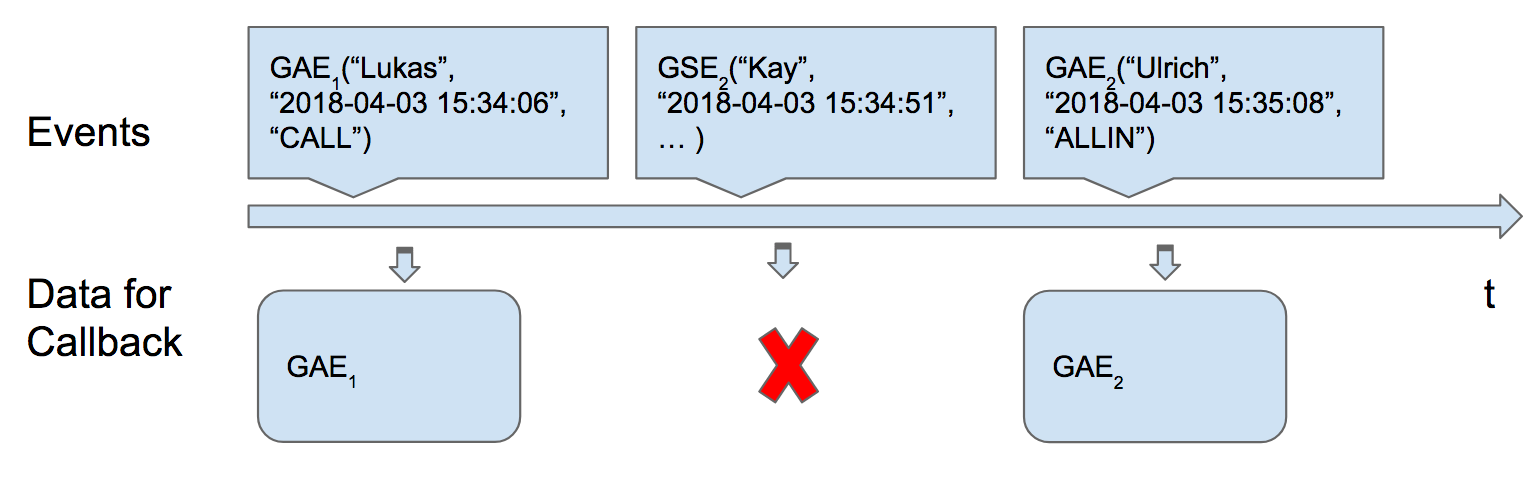
\includegraphics[width=\textwidth,height=\textheight, keepaspectratio]{images/statement_basic_select.png}
	\caption{Ablauf einfache Selektion}
	\label{basic_select_img}
\end{figure}

\section{Filter}

Die Filterfunktion ist eine geeignete Möglichkeit, die Selektion aus dem Ereignisfluss auf bestimmte Attribut-Werte zu beschränken. In Quelltext \ref{filter_select} ist veranschaulicht, wie gleich dem SQL Syntax Ereigniseigenschaften beschränkt werden.
\begin{lstlisting}[caption={Statement mit Filter},label=filter_select,captionpos=b,language=SQL]

select playerName, deck from GameEndEvent(deck="ROYAL_FLUSH")

\end{lstlisting}
Wie der Quellcode \ref{filter_select} zeigt, selektiert die Event-Engine die Attribute \texttt{playerName} und \texttt{deck} der auftretenden Ereignisse vom Typ \texttt{GameEndEvent}. Anschließend wird mit \texttt{GameEndEvent(deck="ROYAL\_FLUSH")} überprüft, ob der Wert des Deck-Attributes im Endevent, einem Royal-Flush entspricht.

Der Ablauf des Quellcodes wird in Abbildung \ref{filter_select_img} aufgezeigt. Gut zu sehen ist, dass nur die End-Events erfasst werden, welche dem Attribut-Wert entsprechen. Weil nur ein Spieler mit einem Royal-Flush-Blatt gewinnt, wird auch nur dieses Ereignis verarbeitet.
Das Casino benötigt ein solches Statement, um zu erfahren, wer welches Spiel mit welcher Hand gewonnen wird. Um jedoch, einen Spieler mit oftmaligem Glück zu entdecken, ist die Anzahl der Siege erwünscht. Hierfür können die selektierten Daten, mit weiteren Funktionen aggregiert werden.
\cite{EsperRef2018}[10-11]

\begin{figure}[ht]
	\centering
	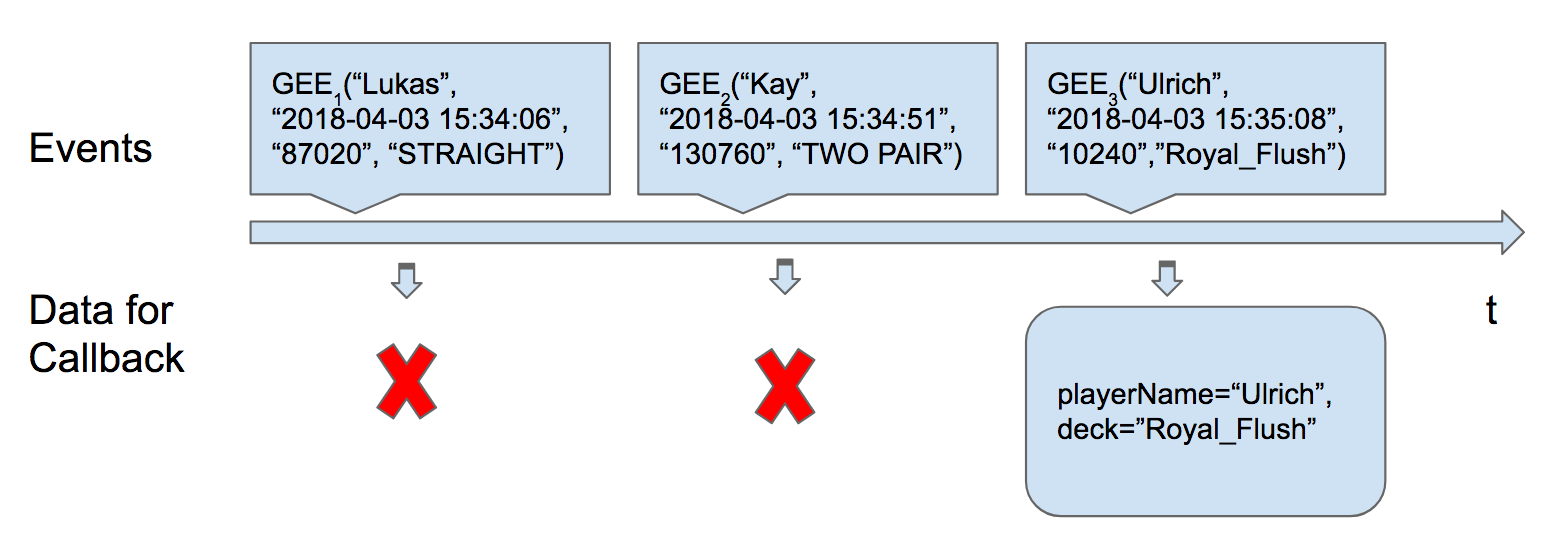
\includegraphics[width=\textwidth,height=\textheight, keepaspectratio]{images/statement_basic_filter.png}
	\caption{Ablauf gefilterte Selektion}
	\label{filter_select_img}
\end{figure}

\section{Aggregation}

Um zu erfahren, welcher Spieler wie oft gewonnen hat wird die Aggregationsfunktion \texttt{count(playerName)} verwendet.
\begin{lstlisting}[caption={Statement mit Aggregation},label=aggregation_select,captionpos=b,language=SQL]

select playerName, count(playerName) as wins, deck from GameEndEvent

\end{lstlisting}
Der Ablauf hierbei ist in Abbildung \ref{aggregation_select_img} veranschaulicht. 
Zudem sind weitere Aggregationsfunktionen in Esper verfügbar.
Ereignisse können mit \texttt{sum()} summiert werden. Der Durchschnitt wird durch \texttt{avg()}, Minimal-, sowie Maximalwert mit \texttt{min()} und \texttt{max()} errechnet. \texttt{count()} gibt die Anzahl der Auftretenden Ereignisse. Mit \texttt{median()}, \texttt{stddev()}, \texttt{avedev()} wird der Median, die Standardabweichung, und die Abweichung zum Mittelwert errechnet.
Im Casino fällt auf, dass sich die Spielenden der Vortage in den zu analysierenden Daten befinden. Um nur die Daten des aktuellen Tages auswerten zu können, sind Beschränkungen des auszuwertenden Ereignisstroms erforderlich. Die \acf{EPL} bietet hierfür sogenannte Data-Windows, welche in Abschnitt \ref{Data-Windows} beschrieben werden.
\cite{EsperRef2018}[9-10]

\begin{figure}[ht]
	\centering
	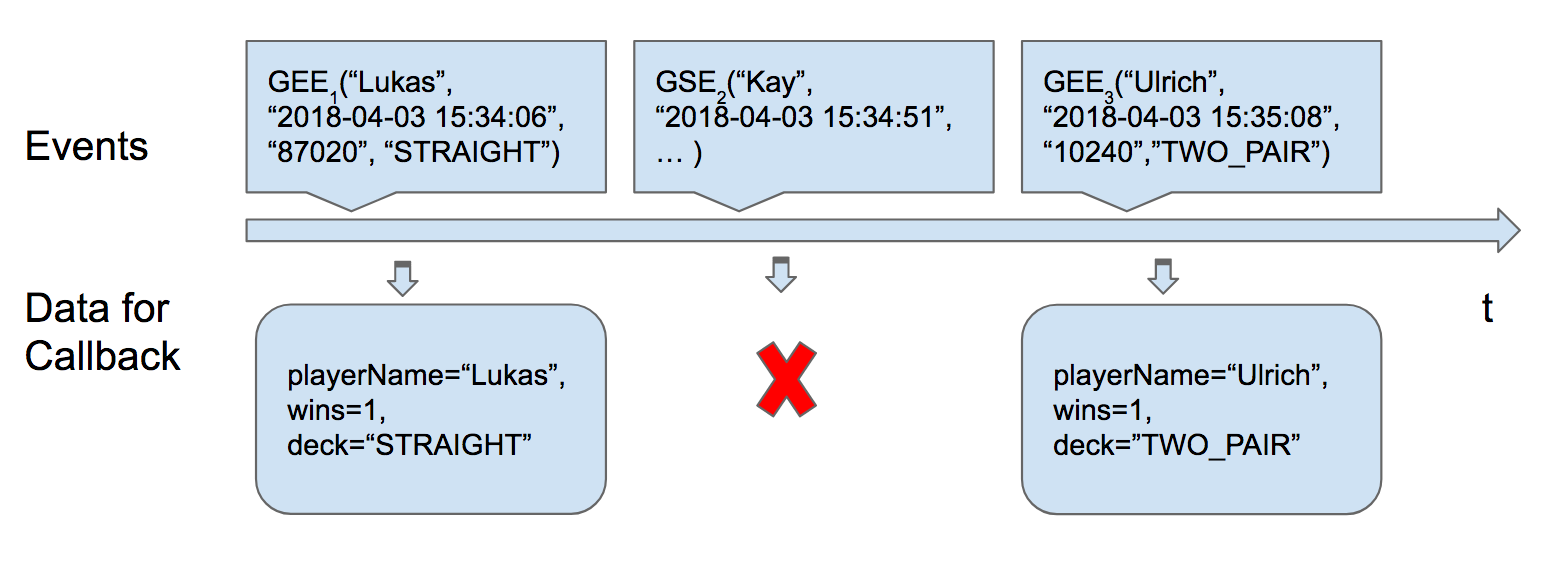
\includegraphics[width=\textwidth,height=\textheight, keepaspectratio]{images/statement_basic_aggregation.png}
	\caption{Ablauf Selektion mit Aggregation}
	\label{aggregation_select_img}
\end{figure}

\section{Data-Windows}
\label{Data-Windows}

\textbf{Data-Windows} werden in Esper verwendet, um Events im Bezug zueinander zu betrachten (Kausalität). Je nach Eigenschaft des \textbf{Data-Windows}, werden sie anhand von Kriterien (z.B. Anzahl oder Zeit) betrachtet.

Ein sehr einfaches \textbf{Data-Window} ist das nachfolgend dargestellte \textbf{Length Window}.

\begin{figure}[ht]
	\centering
	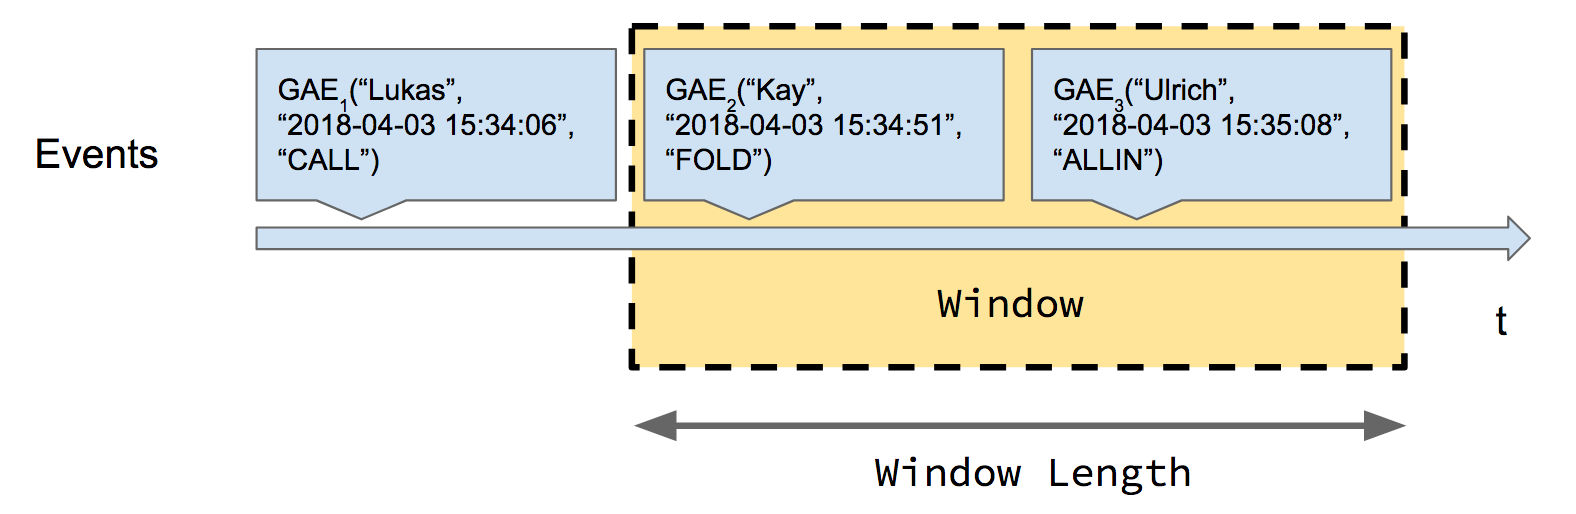
\includegraphics[width=\textwidth,height=\textheight,keepaspectratio]{images/data_window_length.png}
	\caption{Length Window}
	\label{LengthWindow}
\end{figure}

Dieses \textbf{Data-Window} wird mit einer Länge konfiguriert (in der Abbildung, ist der Wert 2), welche angibt, wie viele Events zusätzlich zum aktuellen betrachtet werden sollen. In diesem Fall würde das aktuelle und vorherige Event betrachtet werden.

Die Art des Events wird im Statement angegeben. Für das obige Beispiel könnte dies folgendermaßen aussehen:

\begin{lstlisting}[caption={Statement mit Length Window},label=length_select,captionpos=b,language=SQL]

select * from GameActionEvent.win:length(2)

\end{lstlisting}

Wichtig ist an dieser Stelle anzumerken, dass das Statement des \textbf{Length Windows} erfüllt ist, sobald mindestens ein Event vom Typ \textbf{GameActionEvent} vorhanden ist. Dabei spielt die angegebene Länge keine Rolle. Nur wenn der Event-Strom mehrere passende Events beinhaltet, wird das \textbf{Length Window} ''gefüllt'' bis zu seiner maximalen Länge.

Ein \textbf{Data-Window} mit einem anderen Ansatz, ist das \textbf{Length-Batch Window}:

\begin{figure}[ht]
	\centering
	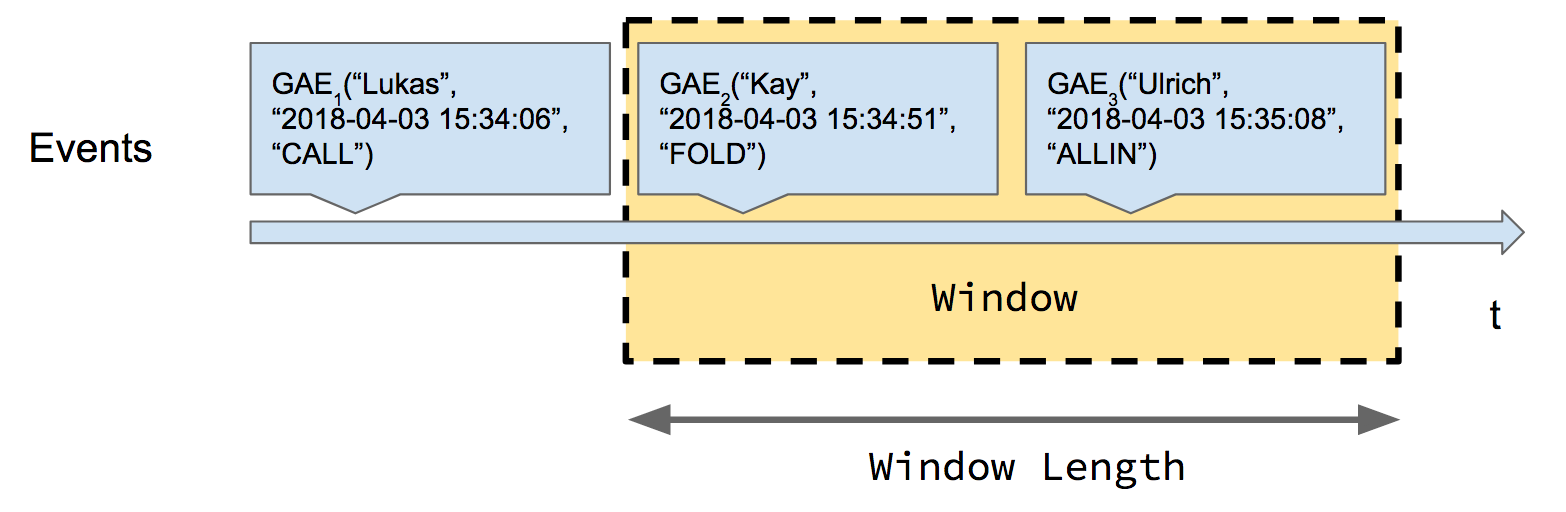
\includegraphics[width=\textwidth,height=\textheight,keepaspectratio]{images/data_window_length_batch.png}
	\caption{Length-Batch Window}
	\label{LengthBatchWindow}
\end{figure}

Dieses \textbf{Data-Window} verhält sich fast identisch zum \textbf{Length Window}, wird allerdings erst erfüllt, wenn genau so viele oder mehr Events im Event-Strom vorhanden sind, wie als Länge des \textbf{Data Windows} angegeben. Dadurch ist es möglich, Abfragen zu erstellen, die zuerst eine gewisse Anzahl an Events benötigen, um eine sinnvolle Weiterverarbeitung zu gewährleisten.

Neben dem betrachten der Anzahl von Events als Kriterium, gibt es auch die Möglichkeit der zeitlichen Betrachtung. Ein Beispiel hierfür ist das \textbf{Time Window}:

\begin{figure}[ht]
	\centering
	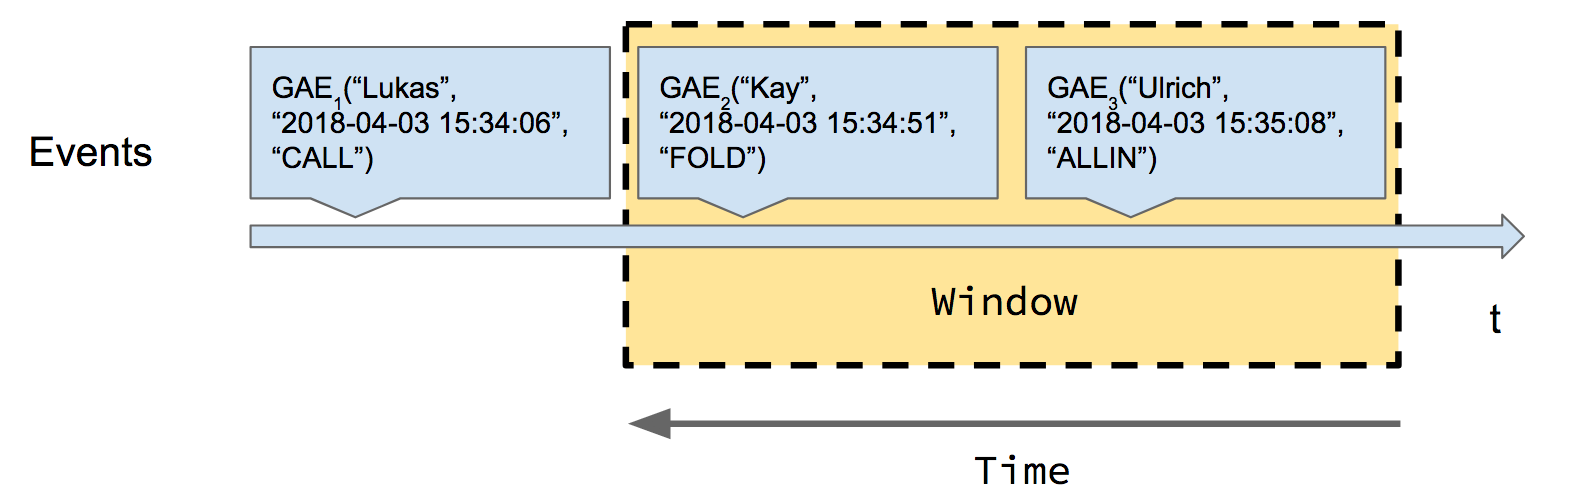
\includegraphics[width=\textwidth,height=\textheight,keepaspectratio]{images/data_window_time.png}
	\caption{Time Window}
	\label{TimeWindow}
\end{figure}

Bei diesem \textbf{Data-Window} werden alle Events innerhalb des konfigurierten Zeitabschnittes betrachtet.
Dabei wird stets vom aktuellen Zeitpunkt aus, anhand des angegeben Zeitwertes (z.B. 5 Sekunden), in die Vergangenheit gegangen. In anderen Worten, würden wir als Ergebnis das aktuelle Event erhalten und alle Events die bis zu 5 Sekunden vorher stattgefunden haben.

Zu Letzt gibt es auch ein \textbf{Data-Window} ohne Kriterium, das \textbf{Keep-All Window}:

\begin{figure}[ht]
	\centering
	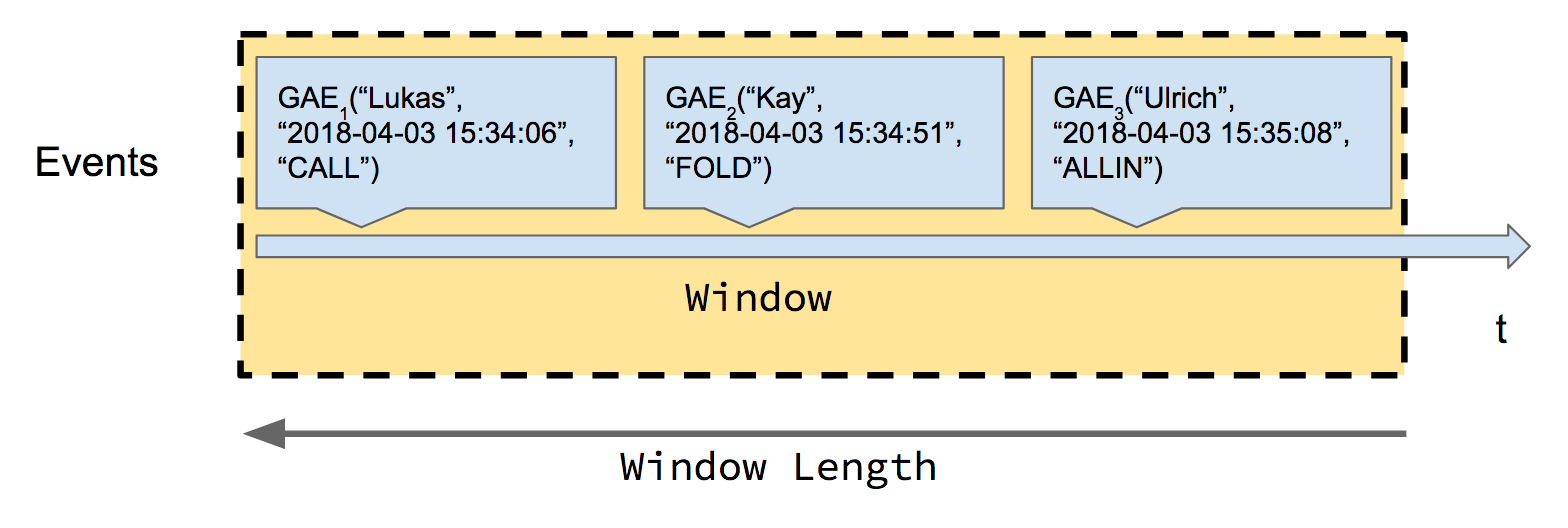
\includegraphics[width=\textwidth,height=\textheight,keepaspectratio]{images/data_window_keep_all.png}
	\caption{Keep-All Window}
	\label{KeepAllWindow}
\end{figure}

Dieses \textbf{Data-Window} ist erfüllt, sobald das erste Event im Event-Storm auftaucht. Es werden beliebig viele Events gesammelt und im Speicher gehalten.
Aufgrund von dem hohen Speicherverbrauch, sollte dieses nur eingesetzt werden, wenn eine kleine Event-Menge vorliegt und diese Gesamt Betracht werden sollen.

\section{Patterns}

Eine Alternative zu den Select-Satements stellen Abfragen nach Strukturen, sogenannte Patterns dar. Events, welche den Bedingungen entsprechen, werden erfasst. Hierbei kommen verschiedene Elemente bei der Pattern-Definition zum Einsatz.
\cite{EsperRef2018}[25]

\begin{enumerate}
	\item \textbf{Kontrolloperator:} \texttt{every} definiert die Erstellung eines Pattern und regelt die Abarbeitung. Es wird alle(engl. every) auf das Ereignismuster zutreffende Ereignisse erfasst. Ein simples Pattern, welches alle Ereignisse vom Typ \texttt{GameActionEvent} erfasst, kann dem nachfolgenden Quellcode entnommen werden.
	Mit der \texttt{where}-Klausel können wie bei der Selektion weitere Bedingungen, definiert werden.
	
	\begin{lstlisting}[caption={Einfaches Pattern mit Where-Klausel},label=basic_pattern, captionpos=b,language=SQL]

	select *
	from patetern [ every GameActionEvent ]
	
	\end{lstlisting}
	
	\item \textbf{Logische Operatoren:} 
	Das Pattern kann, wie im unten dargestellten Quellcode veranschaulicht, durch logische Operatoren wie \texttt{and, or , not} zusammengesetzt werden. Dadurch kann das Ereignismuster mit Bedingungen versehen werden. In diesem Beispiel würden Events vom Typ \texttt{GameEndEvent} oder vom Typ \texttt{GameActionEvent} erfasst werden.
	
	\begin{lstlisting}[caption={Pattern mit logischen Operatoren},label=logic_pattern,captionpos=b,language=SQL]
	
	select *
	from pattern [
	every a=GameActionEvent or b=GameActionEvent ]
	
	\end{lstlisting}
	
	\item \textbf{Nachfolge-Operator:}
	Der Nachfolge-Operator \texttt{->} tritt ein wenn das davor, gefolgt vom danach definierten Ereignis eintrifft. In Quellcode \ref{follow_pattern}  werden alle Endevents betrachtet, welche auf ein Aktionsevent folgen. Die Bedingung trifft zu, wenn der vorangegangene Zug ein Spielausstieg(\texttt{action = "FOLD"}) war.
	Wie im Quellcode zu erkennen ist, werden die Ereignisse in Variablen \texttt{a, b} gespeichert(bspw. \texttt{a=GameAction}). So können die Werte im nächsten Schritt weiterverwendet werden. Im Beispiel wird das Folgeevent (\texttt{b=GameEnd(a.playerName != b.playerName)}) überprüfen ob der Spieler-Name ungleich dem vorherigen ist und im Erfolgsfall erfasst. Auf diese Art lassen sich komplexe bedingte Ereignismuster definieren.
	
	\begin{lstlisting}[caption={Pattern mit Follow-Operator },label=follow_pattern,captionpos=b,language=SQL]
	
	select action, playerName 
	from pattern [every a=GameActionEvent(action="FOLD") 
	-> b=GameEndEvent(a.playerName != b.playerName) ]
	
	\end{lstlisting}
	
	\item \textbf{Bedingungen:}
	Um Grenzen zu definieren, nach welcher das Pattern geprüft wird, dient die \texttt{where}-Klausel. Nach ihr können verschiedene Bedingungen, durch Konstellationen der Operatoren, angegeben werden.
	Meisten werden Vergleichsoperatoren wie \texttt{=, < , > , >=, <=, !=, <>, is null, is not null} und logische Kombinationen wie \texttt{and} oder \texttt{or} verwendet. Ereignisse können hiermit in Korrelation gestellt und ausgewertet werden. Die \texttt{where}- Klausel kann auch bei der Selektion verwendet werden.
	
	\item \textbf{Überwacher} (engl. Observer):
	Um Ereignisströme zu überwachen werden Observer verwendet, welche beispielsweise in einem Zeitintervall oder zu einem Zeitpunkt agieren. Sie können nach der \texttt{where}-Klausel angegeben werden. Beispielsweise kann ein Timer mit Intervall, durch \texttt{timer:interval} definiert werden. Ein Zeitpunkt wird mit \texttt{timer:at} festgelegt, eine Zeitspanne mit \texttt{timer:within}. Für das Casino wird der Überwacher auf ein Zeitintervall eines Werktages gesetzt, um nur die Ereignisse des aktuellen Tages zu erhalten. Historischen Daten fließen somit nicht verfälschend in die Auswertung mit ein.
	
	\begin{lstlisting}[caption={Pattern mit Observer },label=observer_pattern,captionpos=b,language=SQL]
	
	select action, playerName 
	from pattern[ every a=GameActionEvent(action="FOLD") 
	-> b=GameEndEvent(a.playerName != b.playerName) ]
	where timer:within(28800 seconds)
	
	\end{lstlisting}
	
\end{enumerate}

\section{Consumption Modes mit Pattern}

Mit Hilfe der Pattern lassen sich in Esper Consumption Modes umsetzen.
Diese können als Parameterkontexte angesehen werden, welche den Lösungsraum je nach Bedarf einschränken.
Hierzu werden verschiedene Kombinationen des \texttt{every}- und des Nachfolgeoperators, sowie die Prädikatenlogik, genutzt.
Eine Detektion läuft wie folgt ab.
Der Ereignisstrom wird untersucht. Sobald das \textbf{Initiator-Ereignis}, also das vor dem Nachfolgeoperator deklarierte Event, erfasst wird, startet ein Mustererkenner. Dieser sucht nach dem Event, welches als Bedingung hinter dem Nachfolgeoperator deklariert ist. Wird dieses sogenannte \textbf{Detektor-Ereignis} erkannt, gibt der Mustererkenner eine Lösung zurück. Je nach verwendetem Modus kann der Detektor weiterlaufen, oder abbrechen. Zudem können mehrere Mustererkenner parallel arbeiten, wobei der früher gestartete Vorrang erhält.
Ereignisse im Ereignisstrom, welche nicht von Relevanz sind werden \textbf{innere Ereignisse} genannt.
Exakte Erläuterungen zur Prädikatenlogik und damit verbunden logischen Strukturen können \cite{CEP2017}[Anhang 1] entnommen werden.
Der Quelltext \ref{consumption_modes_pattern}[Zeile 2] zeigt einen beispielhaften Ereignisstrom (Zeile 2) von Start-Events (S), End-Events (E) und Action-Events (A). Ebenso zeigt er die verschiedenen Konstellationen von Pattern-Deklarationen zur Umsetzung der Consumption Modes. Anschließend wird die Ergebnismenge angegeben, welche vom jeweiligen Pattern selektiert wird.

\begin{lstlisting}[caption={Pattern Deklaration Consumption Modes},numbers=left,label=consumption_modes_pattern,captionpos=b,language=SQL]
// Ereignisstrom:
// { S1, A1, A2, S2, E1, A3, S3, A4, A5, E2, A6, A7, E3 }

// Continuous
select *
from pattern [ every S -> E ]
// Ergebnismenge: [ {S1, E1}, {S2, E1}, {S3, E2} ]

// Unrestricted
select *
from pattern [ every S -> every E ]
// Ergebnismenge: [ {S1, E1}, {S1, E2}, {S1, E3},
// {S2, E1}, {S2, E2}, {S2, E3}, {S3, E1}, {S3, E2},
// {S3, E3} ]

// Recent-Unique
select *
from pattern [ every (S -> E) ]
// Ergebnismenge: [ {S2, E1}, {S3, E2} ]

// Unnamed
select *
from pattern [ S -> every E ]
// Ergebnismenge: [ {S1, E1}, {S1, E2}, {S1, E3} ]

\end{lstlisting}
Der \textbf{Continuous Consumption-Mode} wird als Pattern mit \texttt{every S -> E} definiert. Dies hat zur Folge, dass der Mustererkenner für jedes auftretende S-Event, das erste darauffolgende E-Event selektiert. 
Hierbei wird jedes Initiator-Ereignis nur einmal verwendet und startet bei Detektion einen eigenen Mustererkenner, welcher bis zum Detektor-Ereignis läuft.
Das Ergebnis für den Continuous Consumption-Mode ist in Quelltext \ref{consumption_modes_pattern}[Zeile 7] erkennbar. \cite{CEP2017}[40-41]
\absatz
Mithilfe des \textbf{Unrestricted Consumption-Mode} lässt sich eine uneingeschränkte Ereignisdetektion durchsetzen. Jedes Initiator-Ereignis
startet einen Mustererkenner, welcher sämtliche passende Detektor-Ereignisse berücksichtigt. Die Mustererkenner laufen parallel nebeneinander.
Dementsprechende sieht die Ergebnismenge wie in Quelltext \ref{consumption_modes_pattern}[Zeile 12-14] aus. \cite{CEP2017}[38]
\absatz
Beim \textbf{Recent-Unique Consumption-Mode} wird,
wie der Name andeutet, nur das letzte bzw. jüngste Initiator-Ereignis verwendet. Dabei gehört ein Detektor- immer nur zu einem Initiator-Ereignis und es existiert nur ein laufender Mustererkenner zur selben Zeit. Dieser wird für jedes Initiator-Ereignis neu gestartet.
Im Gegensatz zum Recent Consumption-Mode wird nicht jedes Detektor- Ereignis bis zum nächsten Initiator berücksichtigt, sondern einzig das zu erst auftretende. Die daraus resultierende Ergebnismenge ist in Quelltext \ref{consumption_modes_pattern}[Zeile 19] aufgezeigt.
\cite{CEP2017}[39-40]
\absatz
Ein weiterer mit Esper umsetzbarer Parameterkontext wird mit \texttt{every (A -> B)} definiert.
Aufgrund fehlender Bezeichnung wir er \textbf{Unnamed Consumption-Mode} genannt.
Die Lösungen werden bei Eintritt des Detektor-Ereignisses erfasst, woraus die Lösungsmenge in Quelltext \ref{consumption_modes_pattern}[Zeile 24] resultiert.
Während der Detektion existiert nur ein Mustererkenner, welcher erst bei einem neuem Initiator-Ereignis neu gestartet wird.
\cite{CEP2017}[35-44, 49-50]

\section{Partitionen}

Esper bietet die Möglichkeit Abfragen zu partitionieren.
Hierzu wird ein zeitlicher Context mit \texttt{create context} erstellt.
\texttt{start} definiert den Start-, \texttt{end} den Endzeitpunkt.
Mit \texttt{after} wir die Dauer auf eine Zeitspanne gesetzt. Verwendet wird der erzeugte Context mit texttt{context OneWorkDay}. Diese Deklaration sorgt dafür, dass sich das darauffolgende \texttt{select}-Statement auf die Partition bezieht.
In Quellcode \ref{partitioned_pattern} wird mit dem ersten Statement eine achtstündige Partition erstellt. Diese wird anschließend durch Angabe vor der Selektion im zweiten Statement verwendet, um die Spieler- und Spielzugnamen aller Aktionen eines Arbeitstagen zu erfassen.
\cite{EsperRef2018}[18]

\begin{lstlisting}[caption={Partitioniertes Pattern},label=partitioned_pattern,captionpos=b,language=SQL]

// Deklaration Kontext
create context OneWorkDay
start @now 
end after 28800 sec

// Verwendung Kontext
context OneWorkDay 
select playerName, action 
from GameActionEvent

\end{lstlisting}
